\chapter{系统实现和工具演示}


\section{\wa 系统实现}
\wa 技术在实验评估中使用 Java 语言实现,并使用 Apache POI 库 \footnote{https://poi.apache.org} 来读写 Excel 格式的电子表格。
相应源码发布在 GitHub 网站上 \footnote{https://github.com/dlee992/QRS19-Code} 。

\wa 工具总共包含约 7,300 行 Java 代码,除了包含 \cu 的源代码以外,额外增改了约 2,500 行代码。
类似于 \cu 的方式,\wa 标记它分析过的电子表格的方法是使用不同的背景色来标注检测到的同一张工作表内的所有单元格类,并通过在单元格右上角添加注释的方式标注含有公式缺陷的单元格的备注信息,包括所在类的信息和具体的公式缺陷种类。


\section{\eg 插件测试工具}
\eg 插件测试工具使用 JavaScript 语言实现,可在 Excel 软件中直接加载并使用的第三方插件,采用 Microsoft Office-js \footnote{https://github.com/OfficeDev/office-js} 框架来异步读写和操作 Excel 文件。
只要是 Excel 可以运行的平台,如 Windows,MacOS 或者浏览器打开相应的 Excel Onedriver 应用中,都可以加载我们的\eg 插件,接近于跨平台兼容。
相应的工具源码发布在 GitHub 上\footnote{https://github.com/dlee992/EGuard}。

目前,\eg 测试工具的实现包含约 3100 行 JavaScript、HTML 和 CSS 代码,其中包含约 2400 行核心功能代码和约 700 行图形界面代码,后续还会继续更新到一个更加完善的版本,然后正式发布上线。

\begin{figure}[tp]   
    \centering
    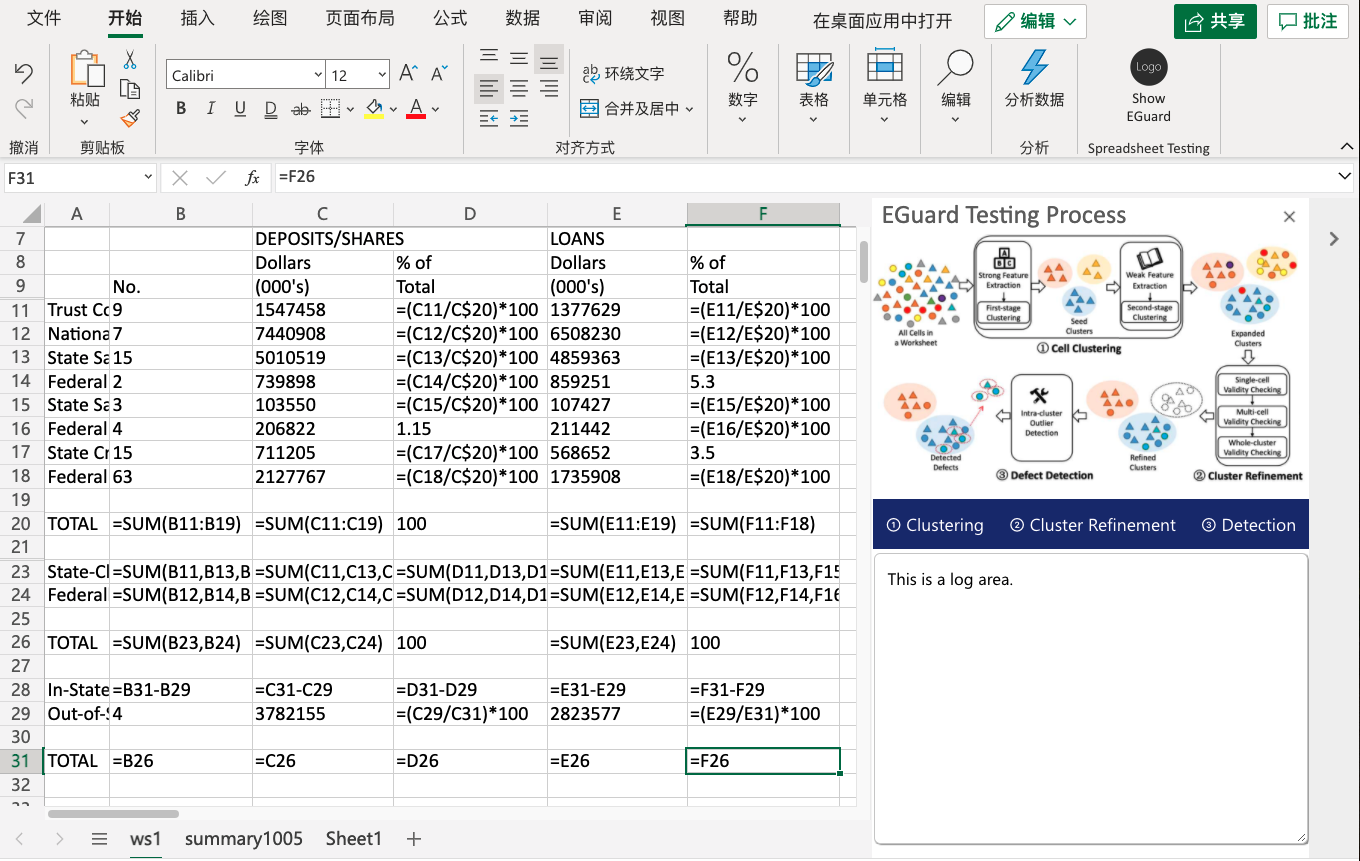
\includegraphics[width=\textwidth]{figure/eg/eguard-1.png}
    \caption{\eg 的插件布局}
    \label{figure-eg1}
\end{figure}
\begin{figure}[tbp]    
    \centering
    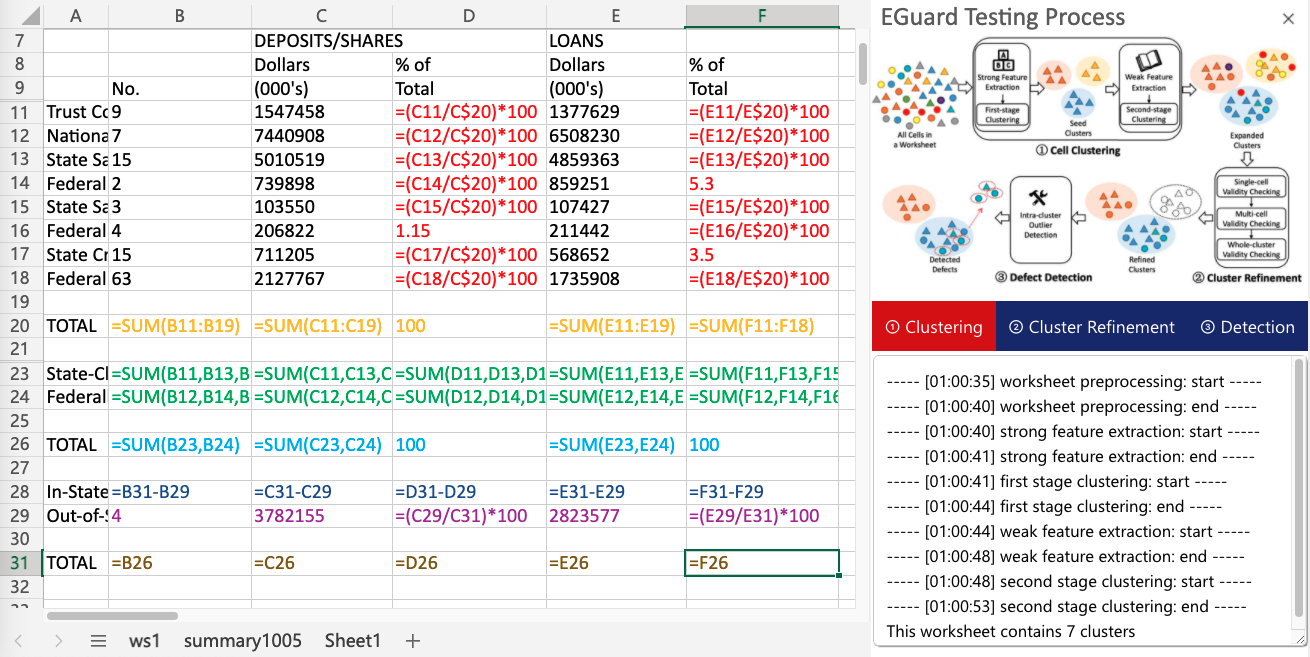
\includegraphics[width=\textwidth]{figure/eg/eguard-2.png}
    \caption{\eg 执行单元格聚类后的电子表格标记和执行信息输出}
    \label{figure-eg2}
\end{figure}
\begin{figure}[tbp]    
    \centering
    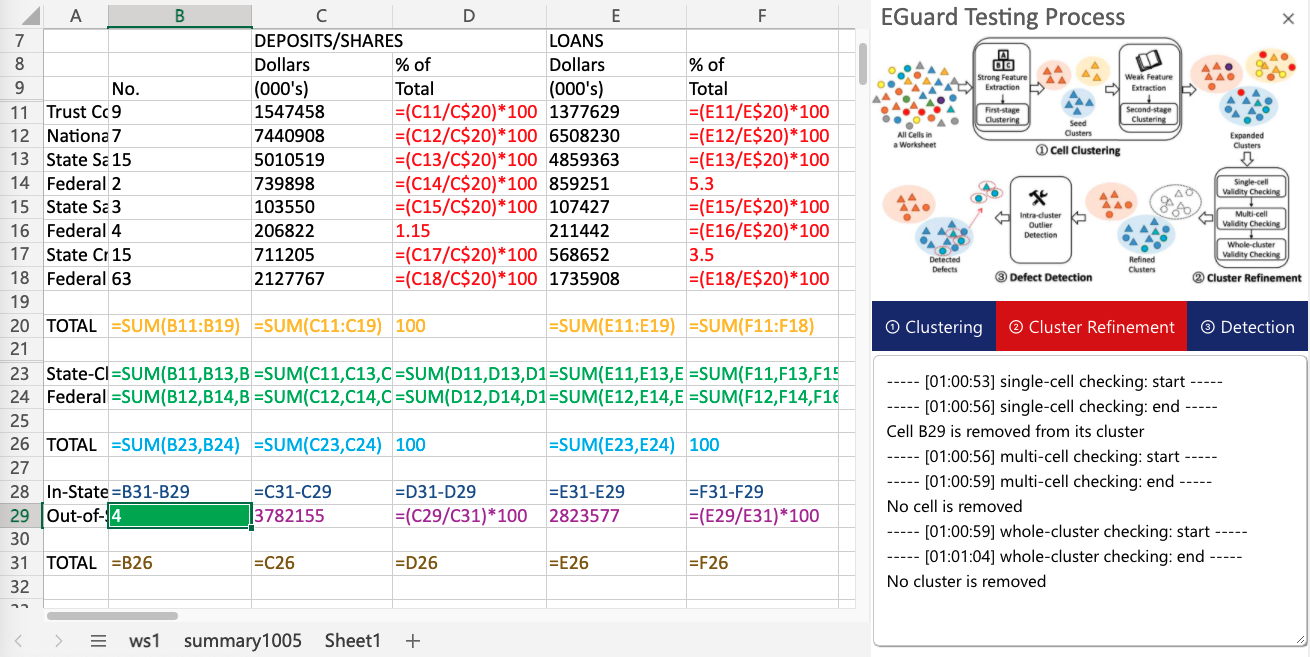
\includegraphics[width=\textwidth]{figure/eg/eguard-3.png}
    \caption{\eg 执行三个单元格检验方法后的电子表格标记和执行信息输出}
    \label{figure-eg3}
\end{figure}
\begin{figure}[tp]   
    \centering
    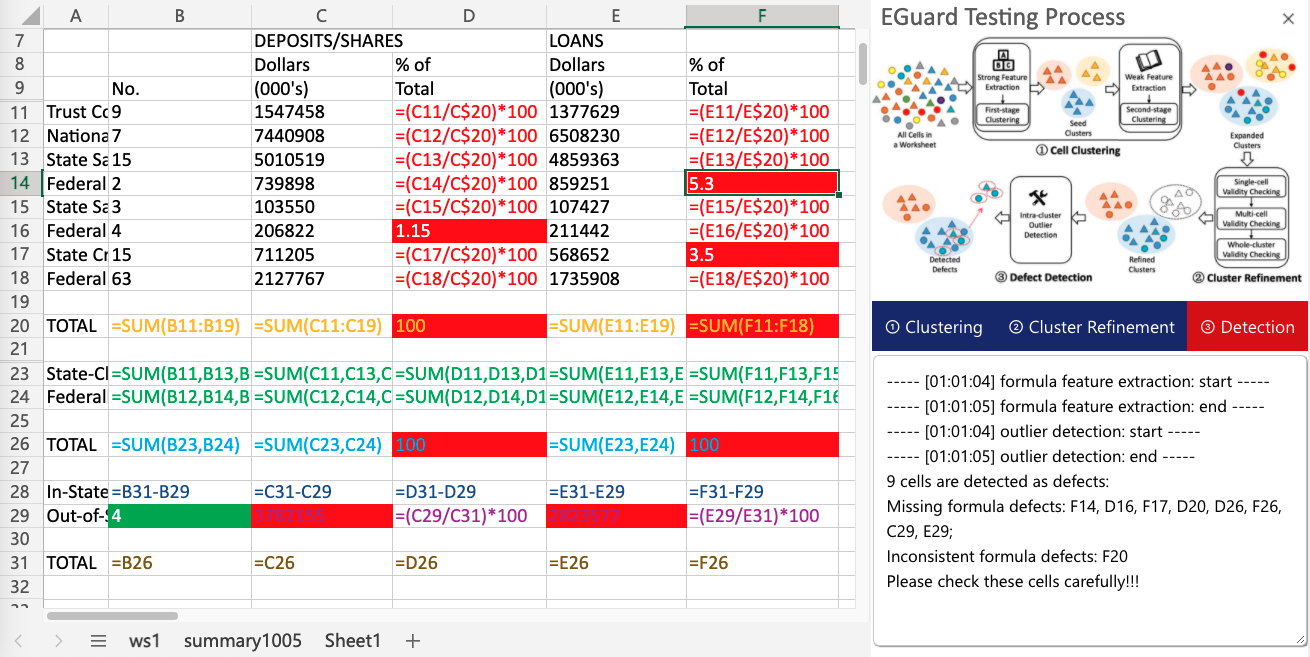
\includegraphics[width=\textwidth]{figure/eg/eguard-4.png}
    \caption{\eg 执行缺陷检测后的电子表格标记和执行信息输出}
    \label{figure-eg4}
\end{figure}

\subsection{界面设计}
如图\ref{figure-eg1}所示,在 Excel 软件中,从“插入”菜单栏选择“Office 加载项”按钮,然后选择本地的插件 \eg 进行加载。
加载完毕后,在“开始”菜单栏的最右侧会显示我们的插件工具图标,点击图标即显示出图\ref{figure-eg1}右侧的内嵌式网页,其标题是“EGuard Testing Process”。
整个内嵌式网页包含如下三个部分:

\begin{enumerate}
    \item 上方显示\eg 插件工具的执行流程图,方便终端用户对检测过程有一个直观感性的认识;
    \item 中间部分为一组选项卡,含有三个执行选项,依次为“\ding{172} Clustering”(两阶段的单元格聚类)、“\ding{173} Cluster Refinement”(基于有效性属性的检验) 和 “\ding{174} Detection”(缺陷检测);
    \item 下方是执行信息输出区域,显示执行的流程和对应的时间戳,以及一些帮助终端用户更好地理解检测结果的辅助信息。
\end{enumerate}

\subsection{使用展示}
接下来,我们结合一个具体的工作表来展示 \eg 的完整使用流程:
\begin{enumerate}
    \item 如图\ref{figure-eg1}所示,首先我们打开一个想要进行测试的 Excel 文件,并切换到想要进行测试的工作表,图中我们打开电子表格“illustrative\_example.xlsx”的工作表“ws1”,按上述方式加载 \eg 插件并在右侧打开嵌入式网页,为了方便观察聚类结果,我们把 Excel 的公式显示选项打开(默认显示 A1 表示法的公式形式);
    
    \item 如图\ref{figure-eg2}所示,点击“\ding{172} Clustering”选项卡按钮,即开始对当前工作表执行强弱特征抽取和两阶段的单元格聚类任务,在插件下方可以看到具体的执行流程包括每个子任务对应的执行时长和一些辅助用户理解的信息。如图所示,最终通过两阶段聚类检测到了 7 个单元格类,并在工作表中用不同的字体颜色标注出来;
    
    \item 如图\ref{figure-eg3}所示,点击“\ding{173} Cluster Refinement”选项卡按钮,即在两阶段聚类的基础上执行针对本文提出的\wa 方法,即第四章描述的 3 种基于有效性属性的检验方法。在当前示例中,依据单个单元格有效性属性检验结果,将单元格 B29 从原先的单元格类 \{B29,C29,D29,E29,F29\} 中移除,因为该单元格并不具备和其他单元格类似的除法运算语义,即如果 B29 具有类似公式,则会显示为=(A29$/$A31)$*$100,但 A29 和 A31 都是字符串单元格,无法进行数值运算。从表中可观察到,被移除的单元格会用绿色背景和白色字体标注出来;
    
    \item 如图\ref{figure-eg4}所示,点击“\ding{174} Detection”选项卡按钮,即在聚类和检验的基础上,进行类内缺陷检测,在当前工作表中,分别从 4 个单元格类中检测出 9 个有缺陷的单元格,其中 8 个为含有常量替换的公式缺陷的单元格,即 F14、D16、F17、D20、D26、F26、C29 和 E29,以及 1 个引用替换的公式缺陷的单元格 F20。从工作表中可观察到,有缺陷的单元格会用红色背景标注出来,如果原来该单元格就是红色字体,为显示结果清晰,则相应改为白色字体,如单元格 D16;
    
    \item 最后,用户可以结合工作表中的标注信息(字体颜色和背景色)和插件下方的日志信息,对工具标记为有公式缺陷的单元格进行检查和修订。
\end{enumerate}


\section{\sg 集成化测试工具}
\sg 工具也是使用 Java 实现的可视化集成工具,同样使用 Apache POI 库来读写 Excel 格式的电子表格。
和\wa 类似,目前只能在 Windows 操作系统下执行。
\sg 的初始核心代码是由张瑞青师兄开发,我们额外添加了两个新技术模块,\cu-OPT\footnote{原\cu 技术的 bug 修复版本} 和 \wa ,并进行了对应的集成编码工作。
相应的工具介绍主页发布在 GitHub Pages 上 \footnote{https://sheetguard.github.io/sguard/},其中包含了工具源码链接和介绍性的视频链接,发布在 YouTube \footnote{https://www.youtube.com/watch?v=gNPmMvQVf5Q} 和 Bilibili \footnote{https://www.bilibili.com/video/BV1x4411g7do} 网站上。

\sg 工具的完整实现包含约 10,500 行 Java 代码,其中包含 7,300 行核心代码和 3,200 行图形界面代码。

\subsection{界面设计}
\begin{figure}[tbp]    
    \centering
    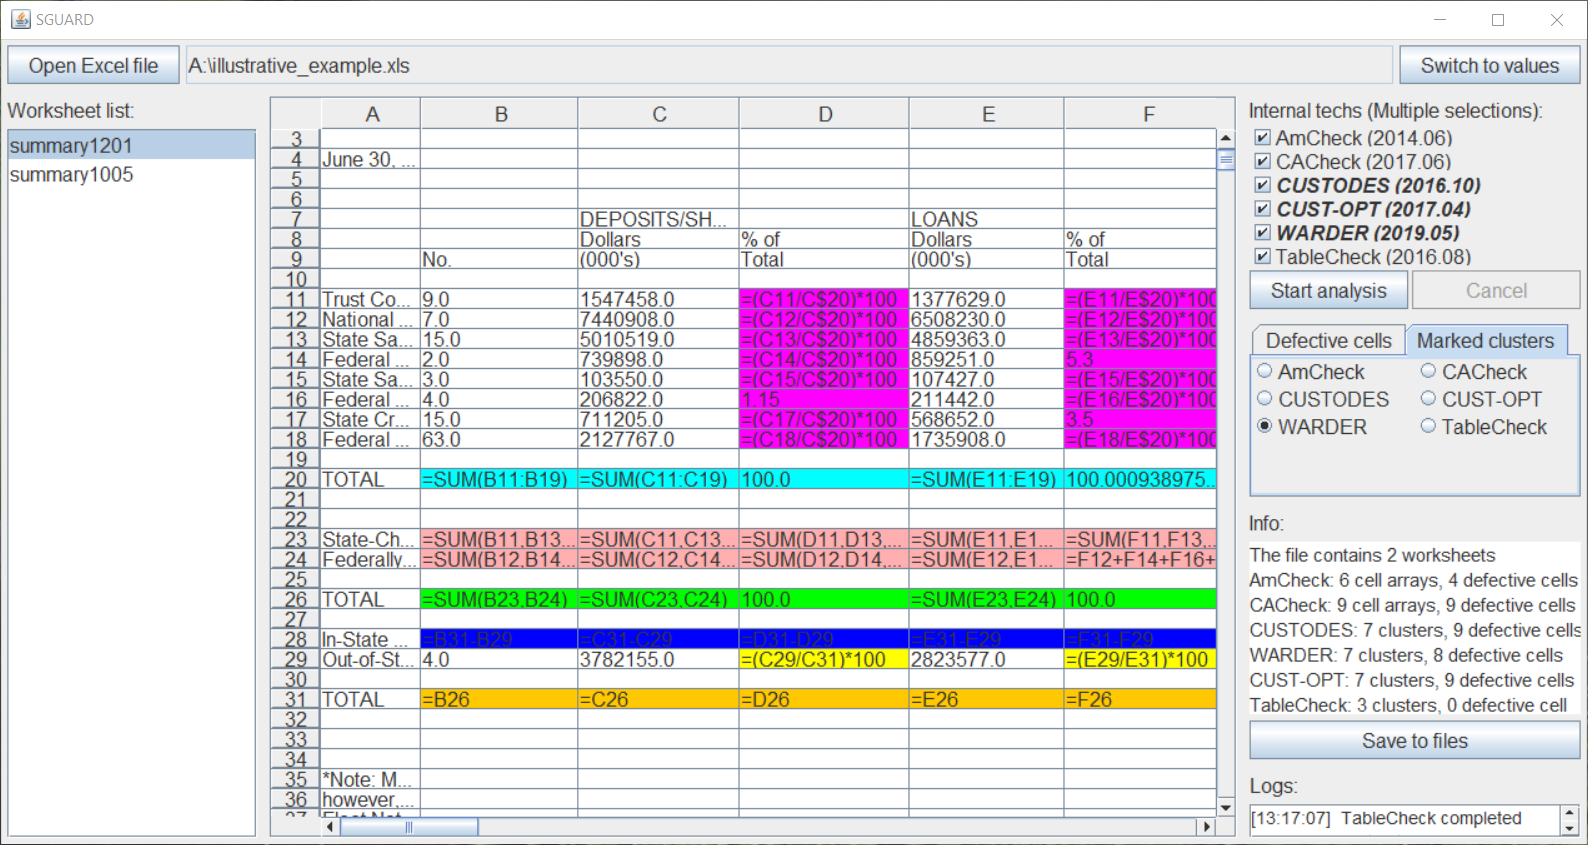
\includegraphics[width=\textwidth]{figure/figure11.png}
    \caption{\sg 的使用截图}
    \label{figure11}
\end{figure}
\begin{figure}[tbp]    
    \centering
    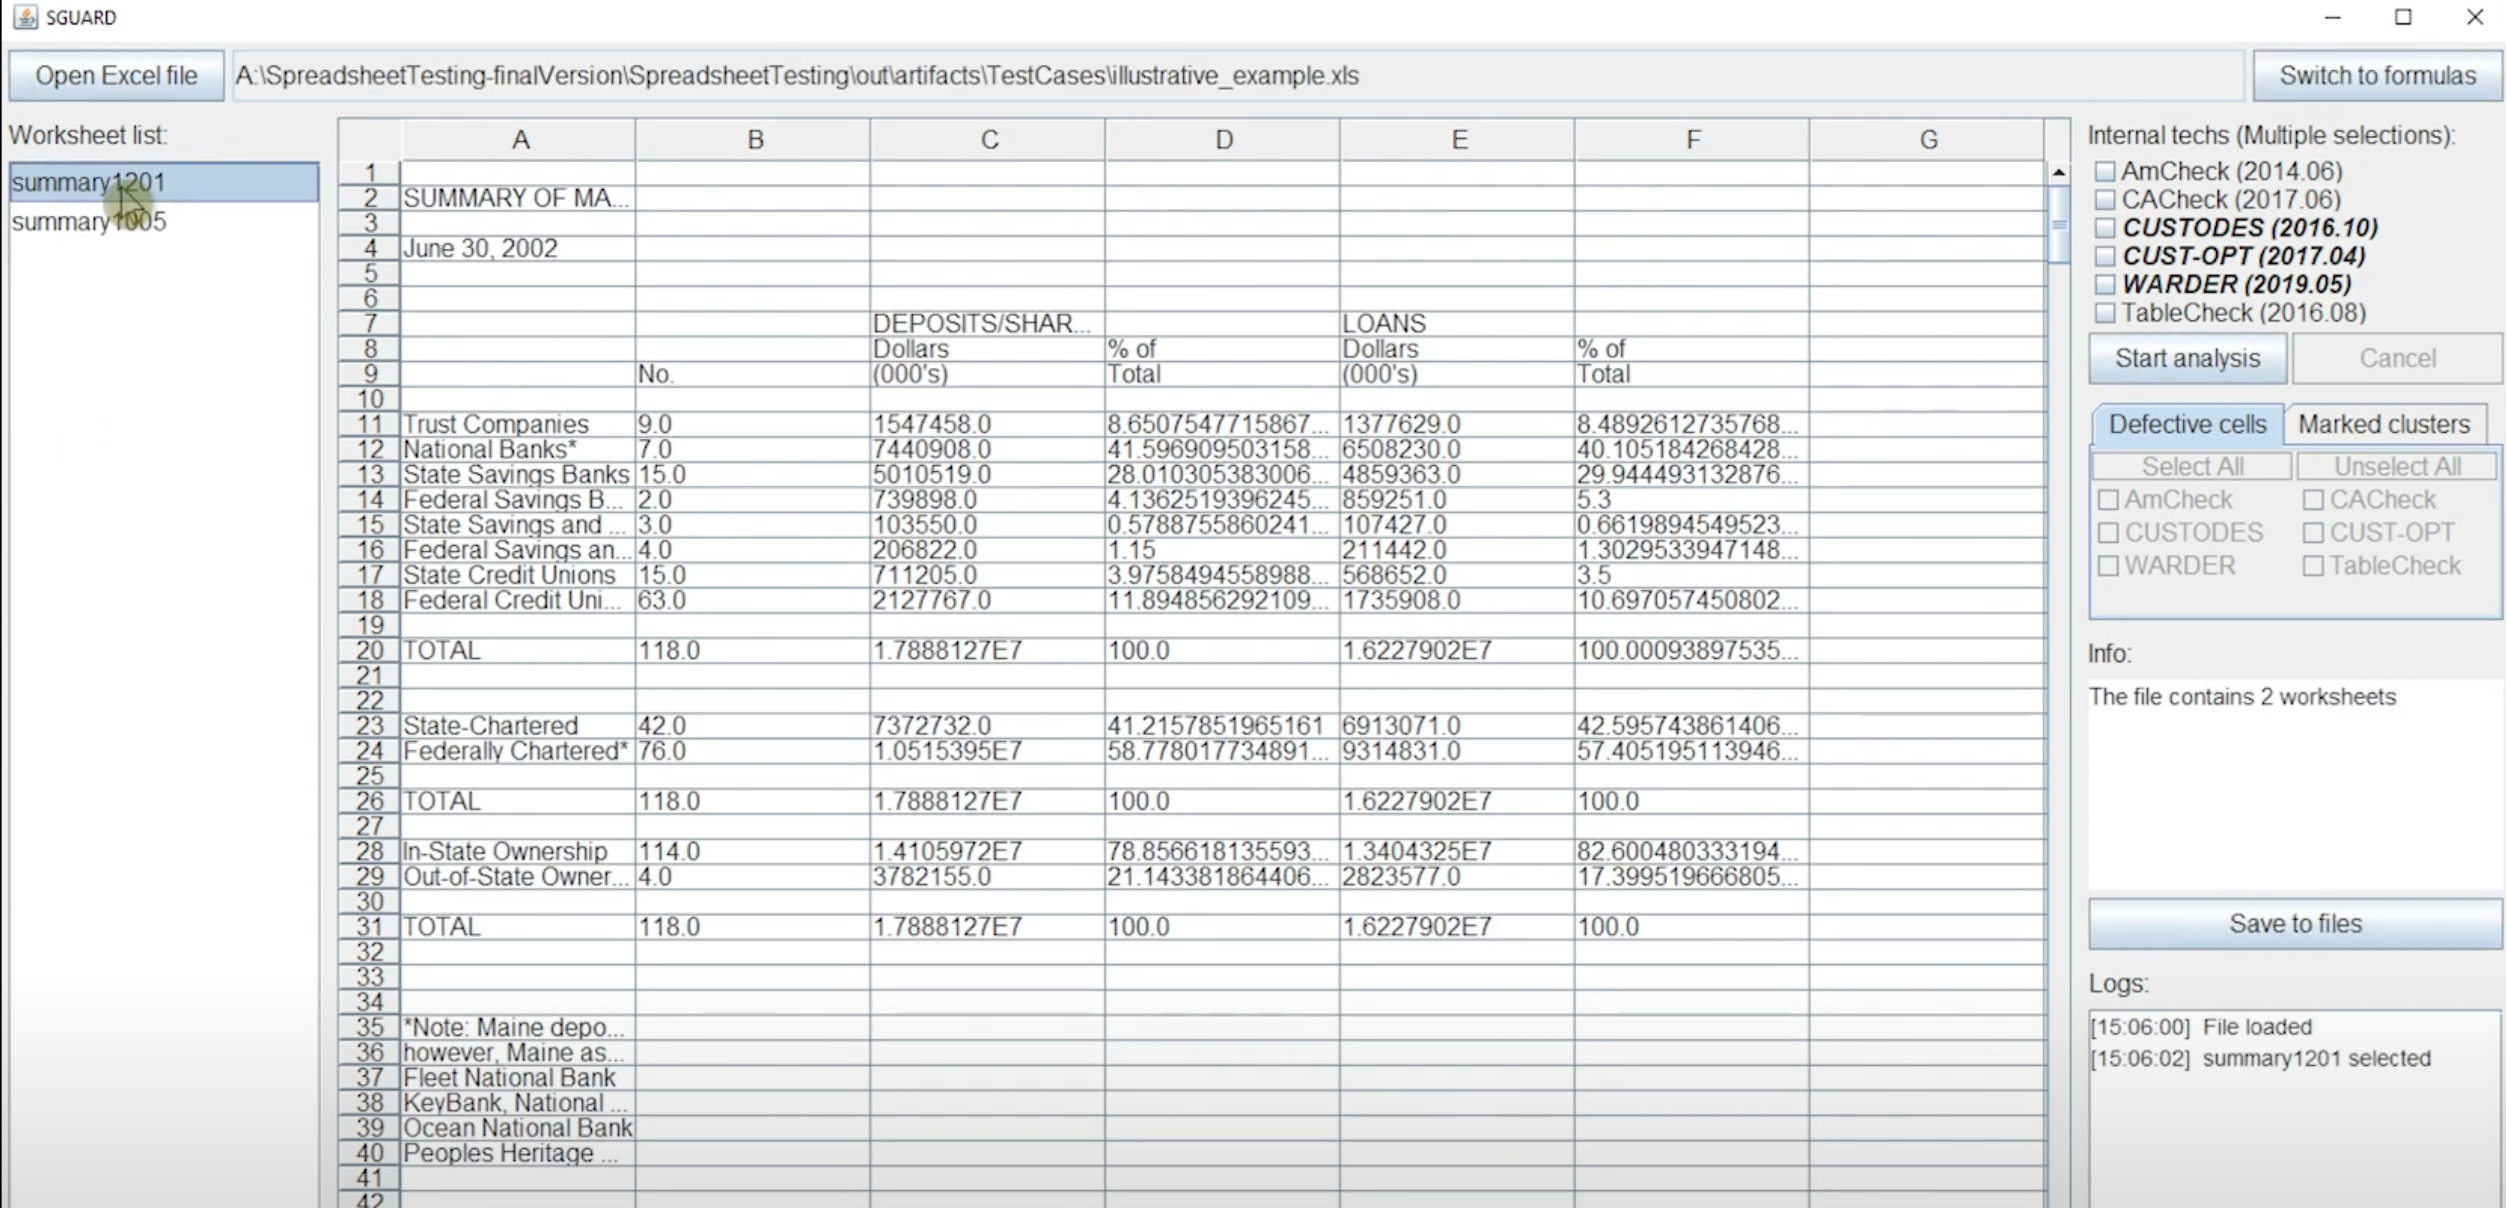
\includegraphics[width=\textwidth]{figure/sg/sguard-3.png}
    \caption{\sg 的使用流程演示截图 3}
    \label{figure-sg3}
\end{figure}
\begin{figure}[tbp]    
    \centering
    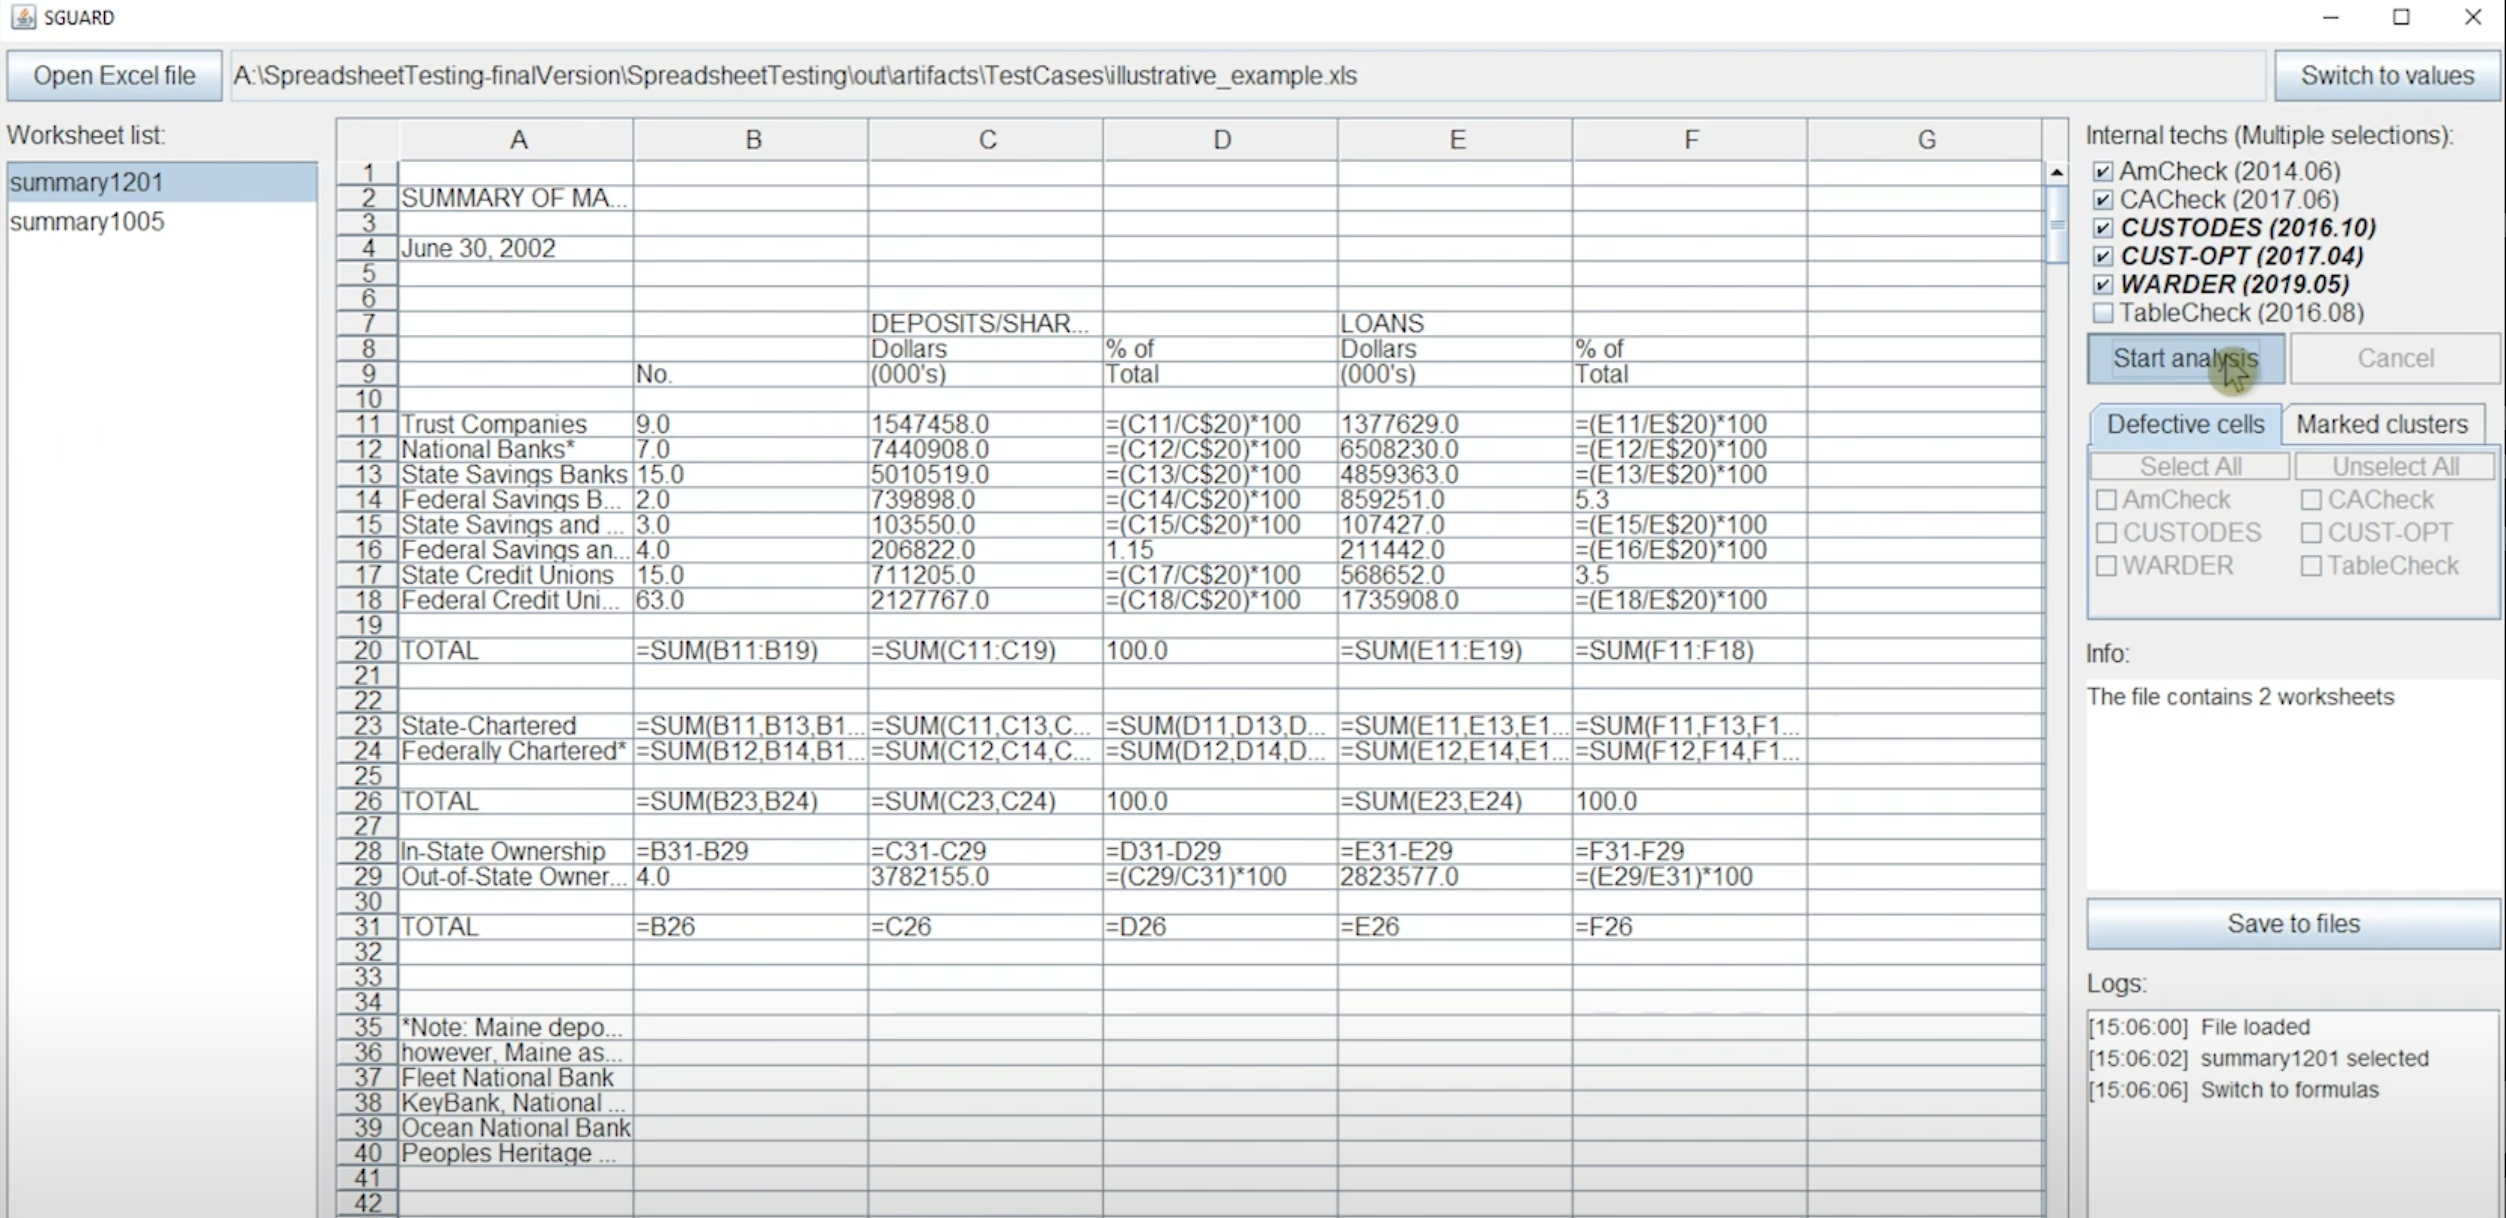
\includegraphics[width=\textwidth]{figure/sg/sguard-4.png}
    \caption{打开待测电子表格并选择待测工作表,再选择要执行的缺陷检测技术并开始执行}
    \label{figure-sg4}
\end{figure}
\begin{figure}[tbp]    
    \centering
    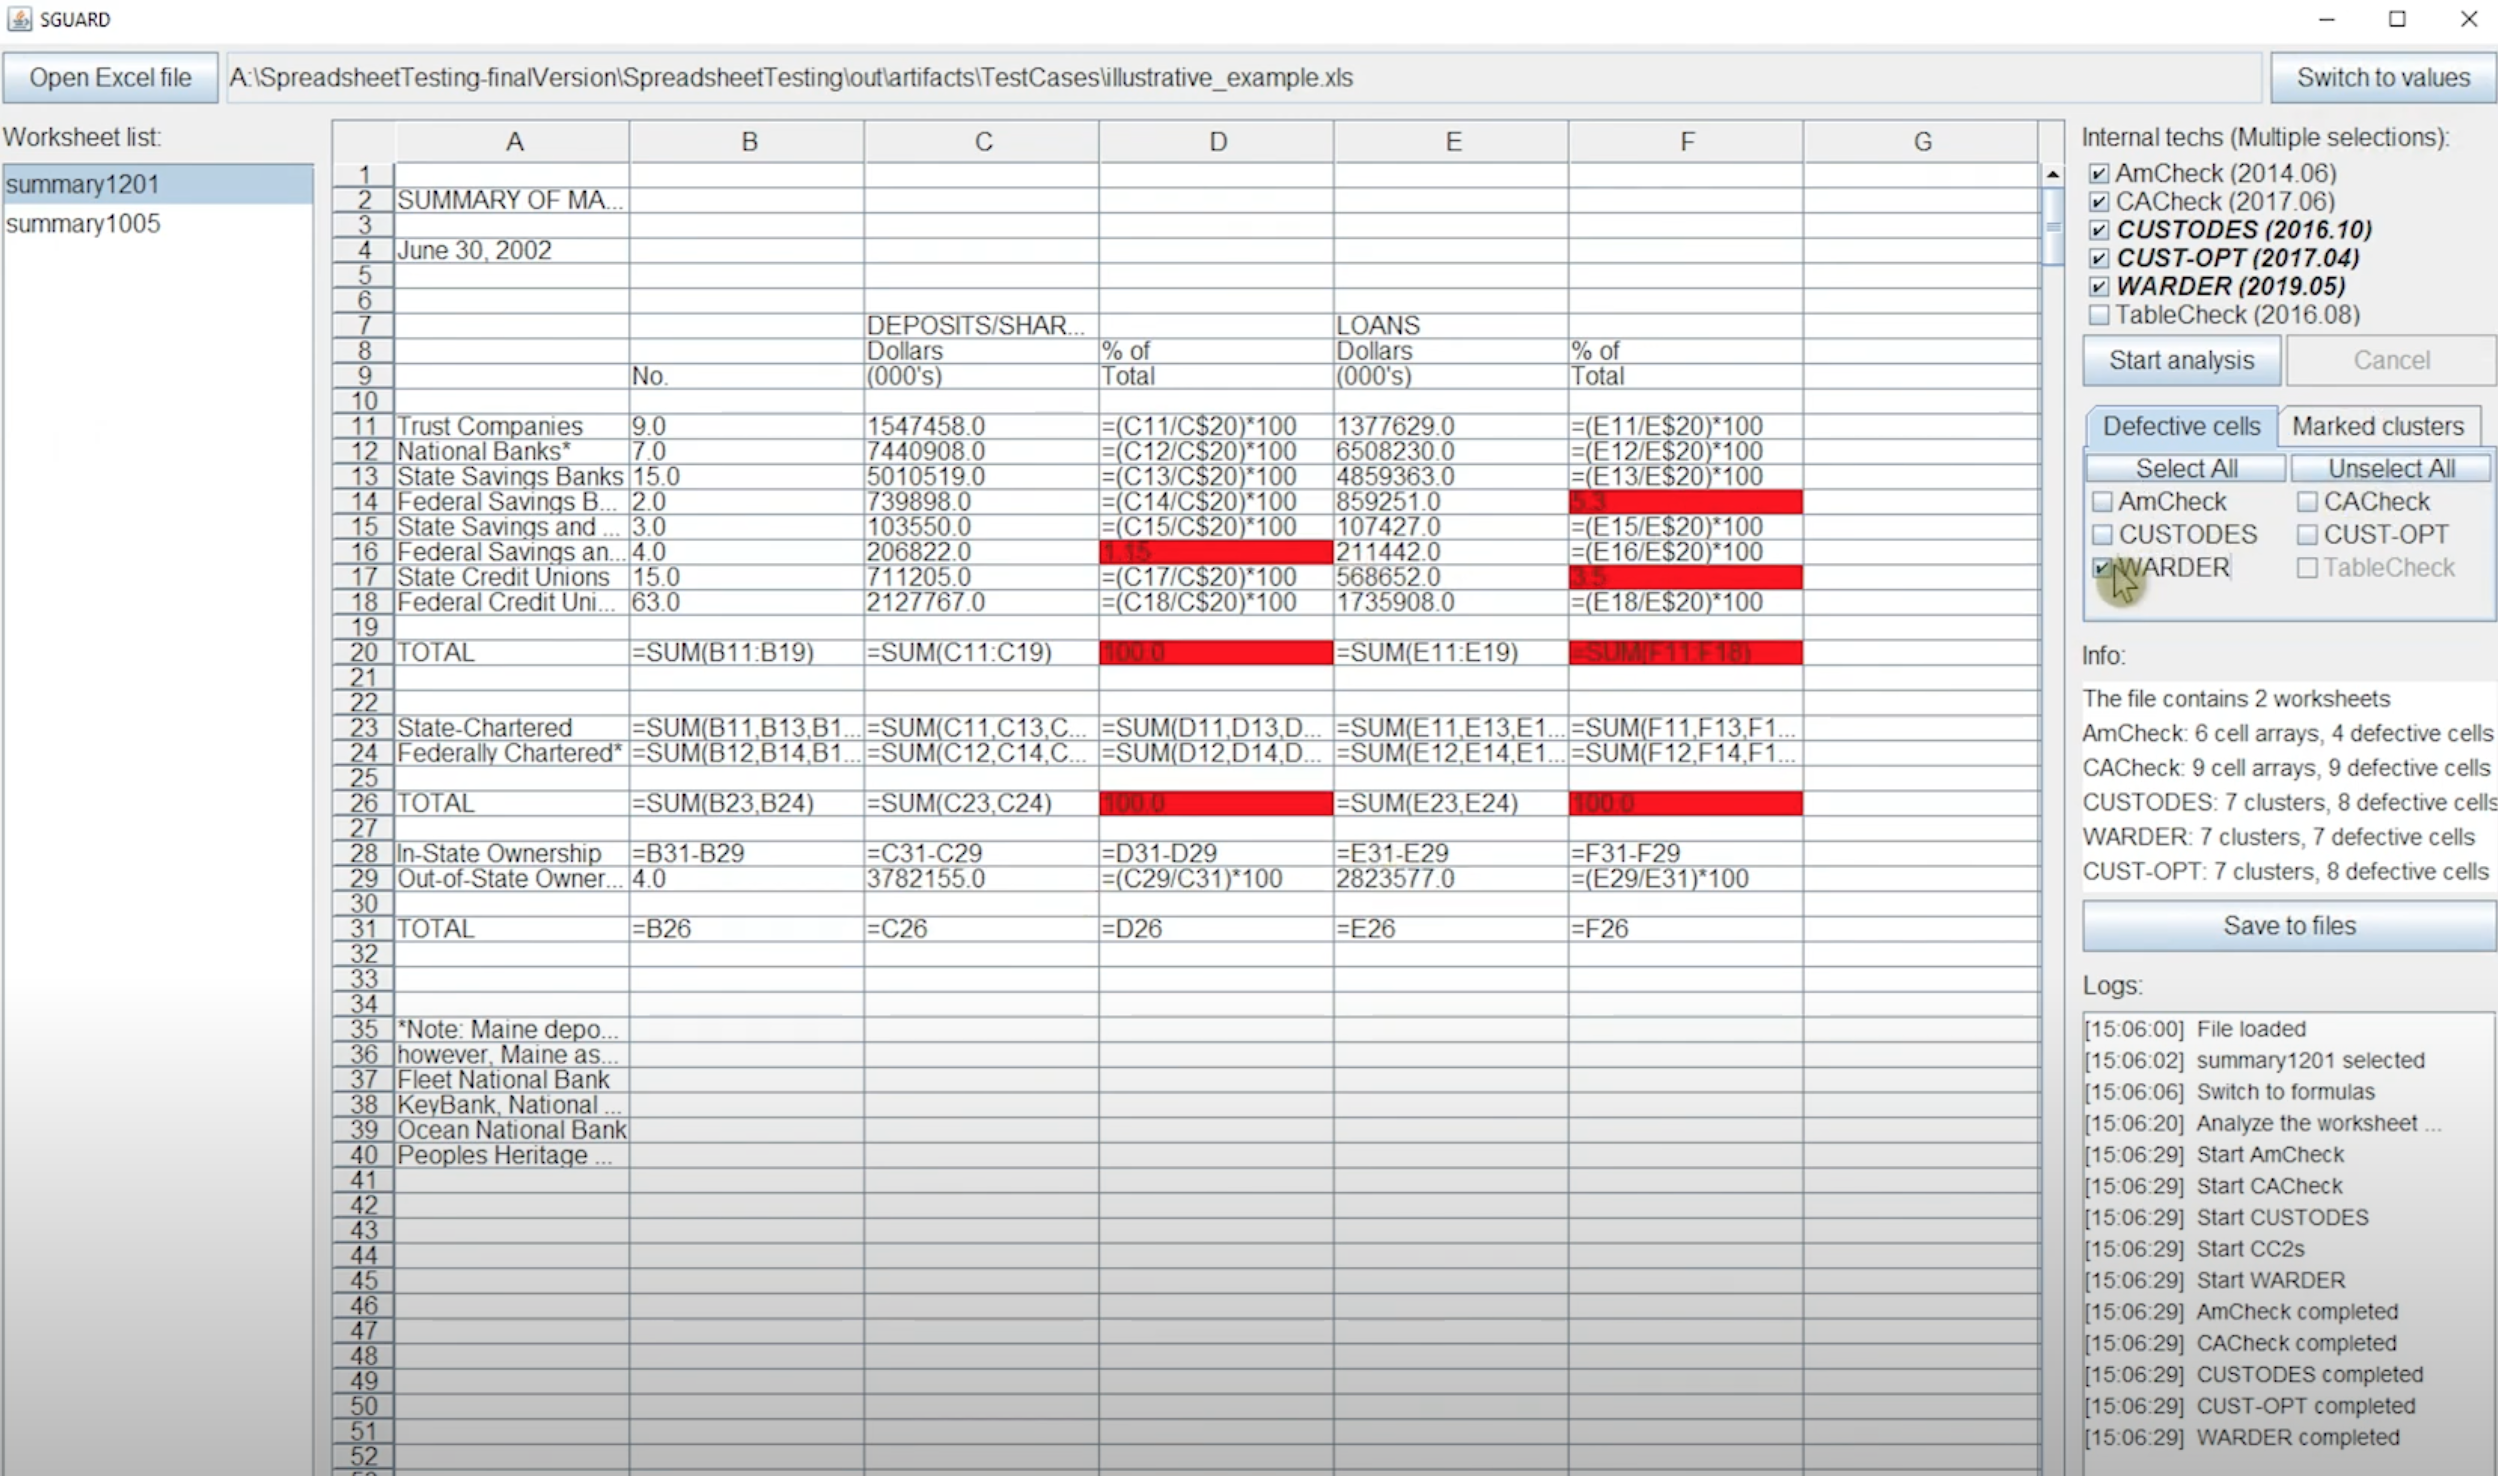
\includegraphics[width=\textwidth]{figure/sg/sguard-5.png}
    \caption{\sg 的使用流程演示截图 5}
    \label{figure-sg5}
\end{figure}
\begin{figure}[tbp]    
    \centering
    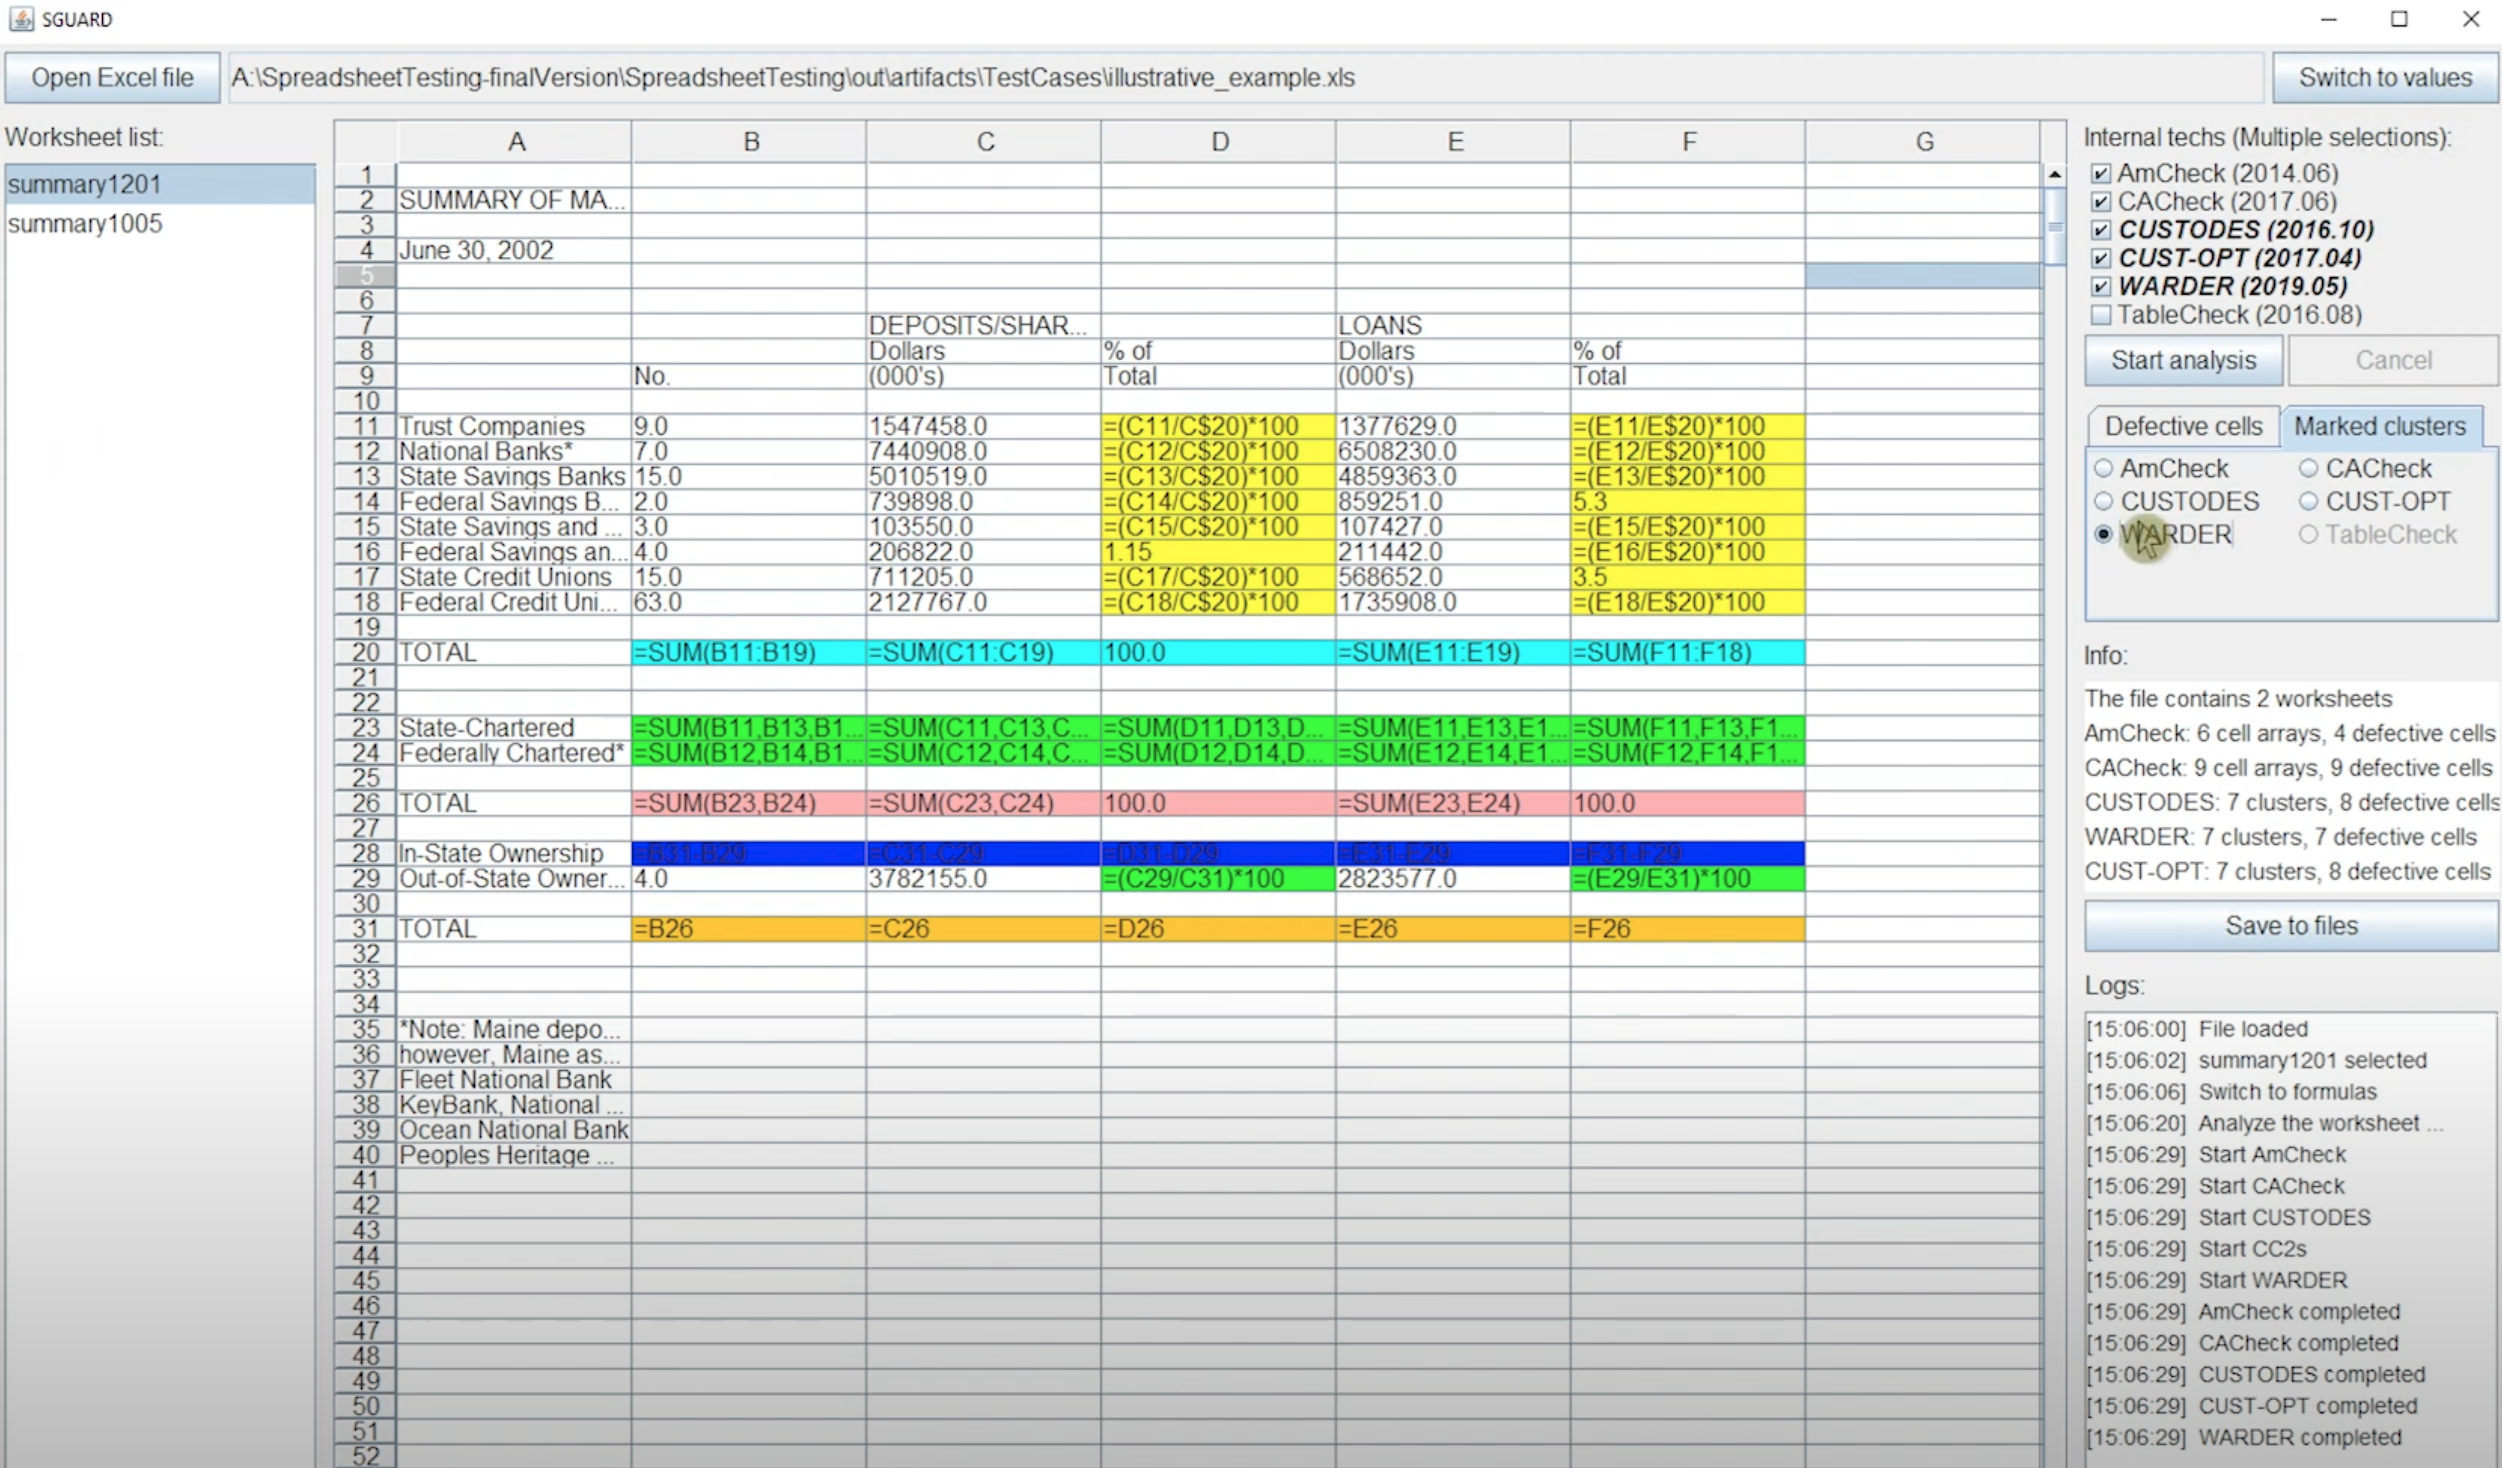
\includegraphics[width=\textwidth]{figure/sg/sguard-6.png}
    \caption{查看 \wa 技术的单元格聚类结果}
    \label{figure-sg6}
\end{figure}
% \begin{figure}[tp]    
    \centering
    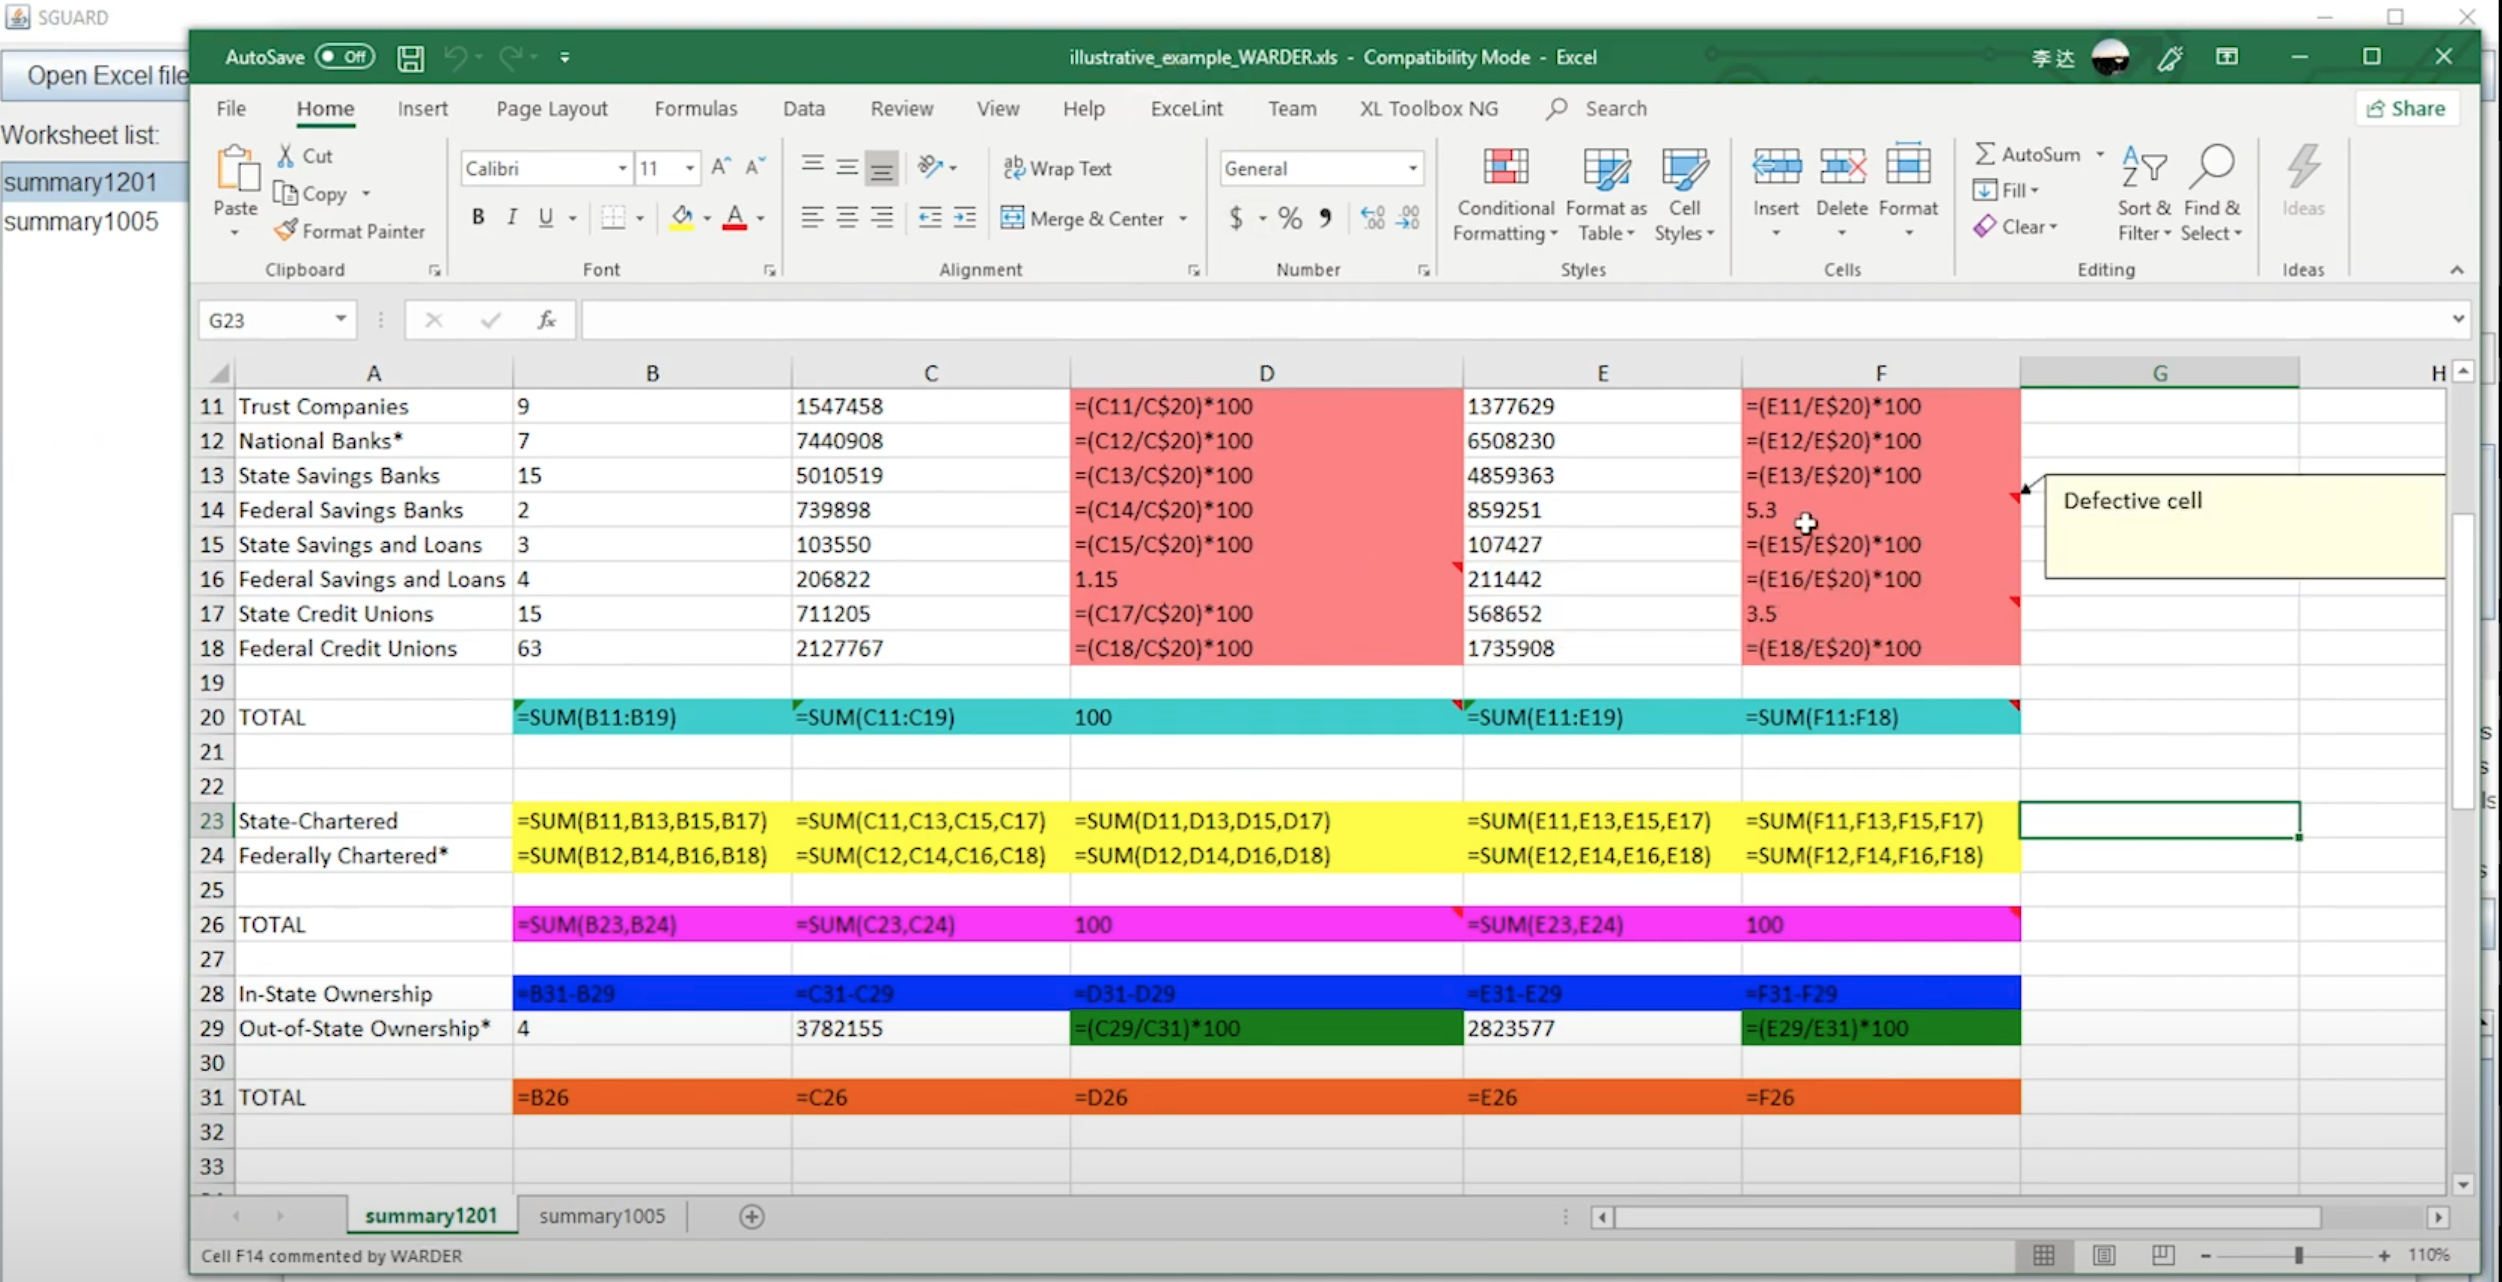
\includegraphics[width=\textwidth]{figure/sg/sguard-8.png}
    \caption{在 Excel 中查看保存好的 \wa 检测结果}
    \label{figure-sg8}
\end{figure}
图\ref{figure11} 展示了\sg 使用交互界面来检测电子表格缺陷并展示相应结果的截图。
整个界面包含四大区域:

\begin{itemize}
    \item 上方的文件选取区域包含 Open Excel file(打开 Excel 文件)和Switch to values/formulas(切换到数值/公式形式)两个按钮,中间部分显示当前打开的 Excel 文件路径;
    
    \item 左侧的工作表选择区域列出了当前选定的 Excel 文件的所有工作表;
    
    \item 中间的工作表内容展示区域展示了类似于电子表格软件的核心界面,即以字母标记的列号(A,B,\dots)和以数字标记的行号(1,2,\dots),每个对应的表格位置显示该工作表的具体内容,即公式、数值或文本,目前不能显示除此以外的内容,比如工作表中插入的图,以及不会保留原工作表的排版风格,只显示每个单元格里的具体内容;
    
    \item 右侧的核心操作区域包含如下几块内容:

        \begin{enumerate}
            \item 上方罗列了 \sg 工具内部囊括的所有检测技术,共有 6 个检测技术,分别是 \am\cite{dou2014spreadsheet},\ca\cite{dou2017cacheck},\cu\cite{cheung2016custodes},\cu-OPT\footnote{http://sccpu2.cse.ust.hk/custodes/cc2s.html},\wa 和 TableCheck\cite{dou2016detecting}。每个技术名称后面标记了对应论文发表的时间或者该技术更新的最新时间;
            
            \item 紧接着向下是 Start analysis 和 Cancel 两个按钮,分别用来开始执行技术对应的代码和取消当前分析过程;
            
            \item 再往下有两个标签,Detective cells 和 Marked clusters,每个运行的技术分别对应标签内部的一个选项;
            
            \item 再往下是 Info 栏,展示一些执行信息以及每个电子表格缺陷检测结果汇总,包含每个技术检测到的单元格类数量和有缺陷的单元格数量;
            
            \item 紧接着是一个 Save to files 按钮,可以用来保存当前选定技术的检测结果到新的 Excel 文件中;
            
            \item 最后是 Logs 栏,用来显示每个完成执行的技术和对应的时间戳。
        \end{enumerate}

\end{itemize}

\subsection{使用展示}
接下来,我们结合一个具体的工作表来展示 \sg 的完整使用流程。

\begin{enumerate}
    \item 我们点击 Open Excel file 按钮,从文件浏览器中选择一个要测试的电子表格,这里我们选择一个电子表格文件illustrative\_example.xls;
    
    \item 如图\ref{figure-sg3}所示,从左侧列出的工作表中,我们选择名为 summary1201 的工作表,对应的单元格内容就自动显示在正中间;
    
    \item 如图\ref{figure-sg4}所示,我们在右侧功能区选择准备使用的电子表格测试技术,这里我们勾选上除 TableCheck 之外的所有技术,并点击 Start analysis 开始执行;
    
    \item 如图\ref{figure-sg5}所示,我们会在 Logs 区域看到各个技术开始和结束的标志,在 Defective cells 选项卡里可以勾选上多个技术,查看对应检测到的缺陷单元格全集,这里我们选择 \wa 技术,可以看到 \wa 检测到了 7 个缺陷单元格,与 Info 区域显示的检测结果保持一致;
    
    \item 如图\ref{figure-sg6}所示,我们在 Marked clusters 选项卡里也可以勾选多个技术,这里我们选择\wa 技术,中间区域显示出\wa 检测到的 7 个单元格类,与 Info 区域显示的检测结果保持一致;
    
    \item 我们点击 Save to files 按钮之后,每个技术的检测结果单独生成一个 Excel 文件,和源文件放在同一个目录下;
    
    % \item 如图\ref{figure-sg8}所示,
    \item 我们点开任意一个工具标注的 Excel 文件,这里我们打开 illustrave\_example\_WARDER.xls 文件,该文件中标注了和 \sg 工具中显示的相同的单元格类,以及在右上角用注释的方式标注出有公式缺陷的单元格。
\end{enumerate}